\subsection{Tổng quan kiến trúc ứng dụng}
\label{sec:implemented-architecture}

\subsubsection{Tổ chức ứng dụng theo MVVM, Repository và Model}
BroomSharing sử dụng Java và XML theo mô hình MVVM + Repository + Model. XML định nghĩa bố cục; Activity và Adapter hiển thị dữ liệu, tiếp nhận thao tác. ViewModel giữ trạng thái màn hình qua LiveData, Repository truy cập Firestore và các dịch vụ mạng, còn Model biểu diễn các đối tượng như Room và Booking. Cách phân chia này tách giao diện khỏi xử lý dữ liệu \parencite{android_views,android_data,broomsharing_source}.

Hình~\ref{fig:mvvm} thể hiện luồng tương tác giữa các thành phần và dịch vụ ngoài. Authentication quản lý danh tính, Firestore lưu nghiệp vụ, Cloudinary lưu ảnh; bản đồ kết hợp MapLibre, MapTiler và openrouteservice. Backend Java kết nối payOS để tạo và đối soát giao dịch. Biểu tượng trong hình sử dụng bộ Fluent UI System Icons \parencite{fluent_system_icons}.

\begin{figure}[H]
\centering
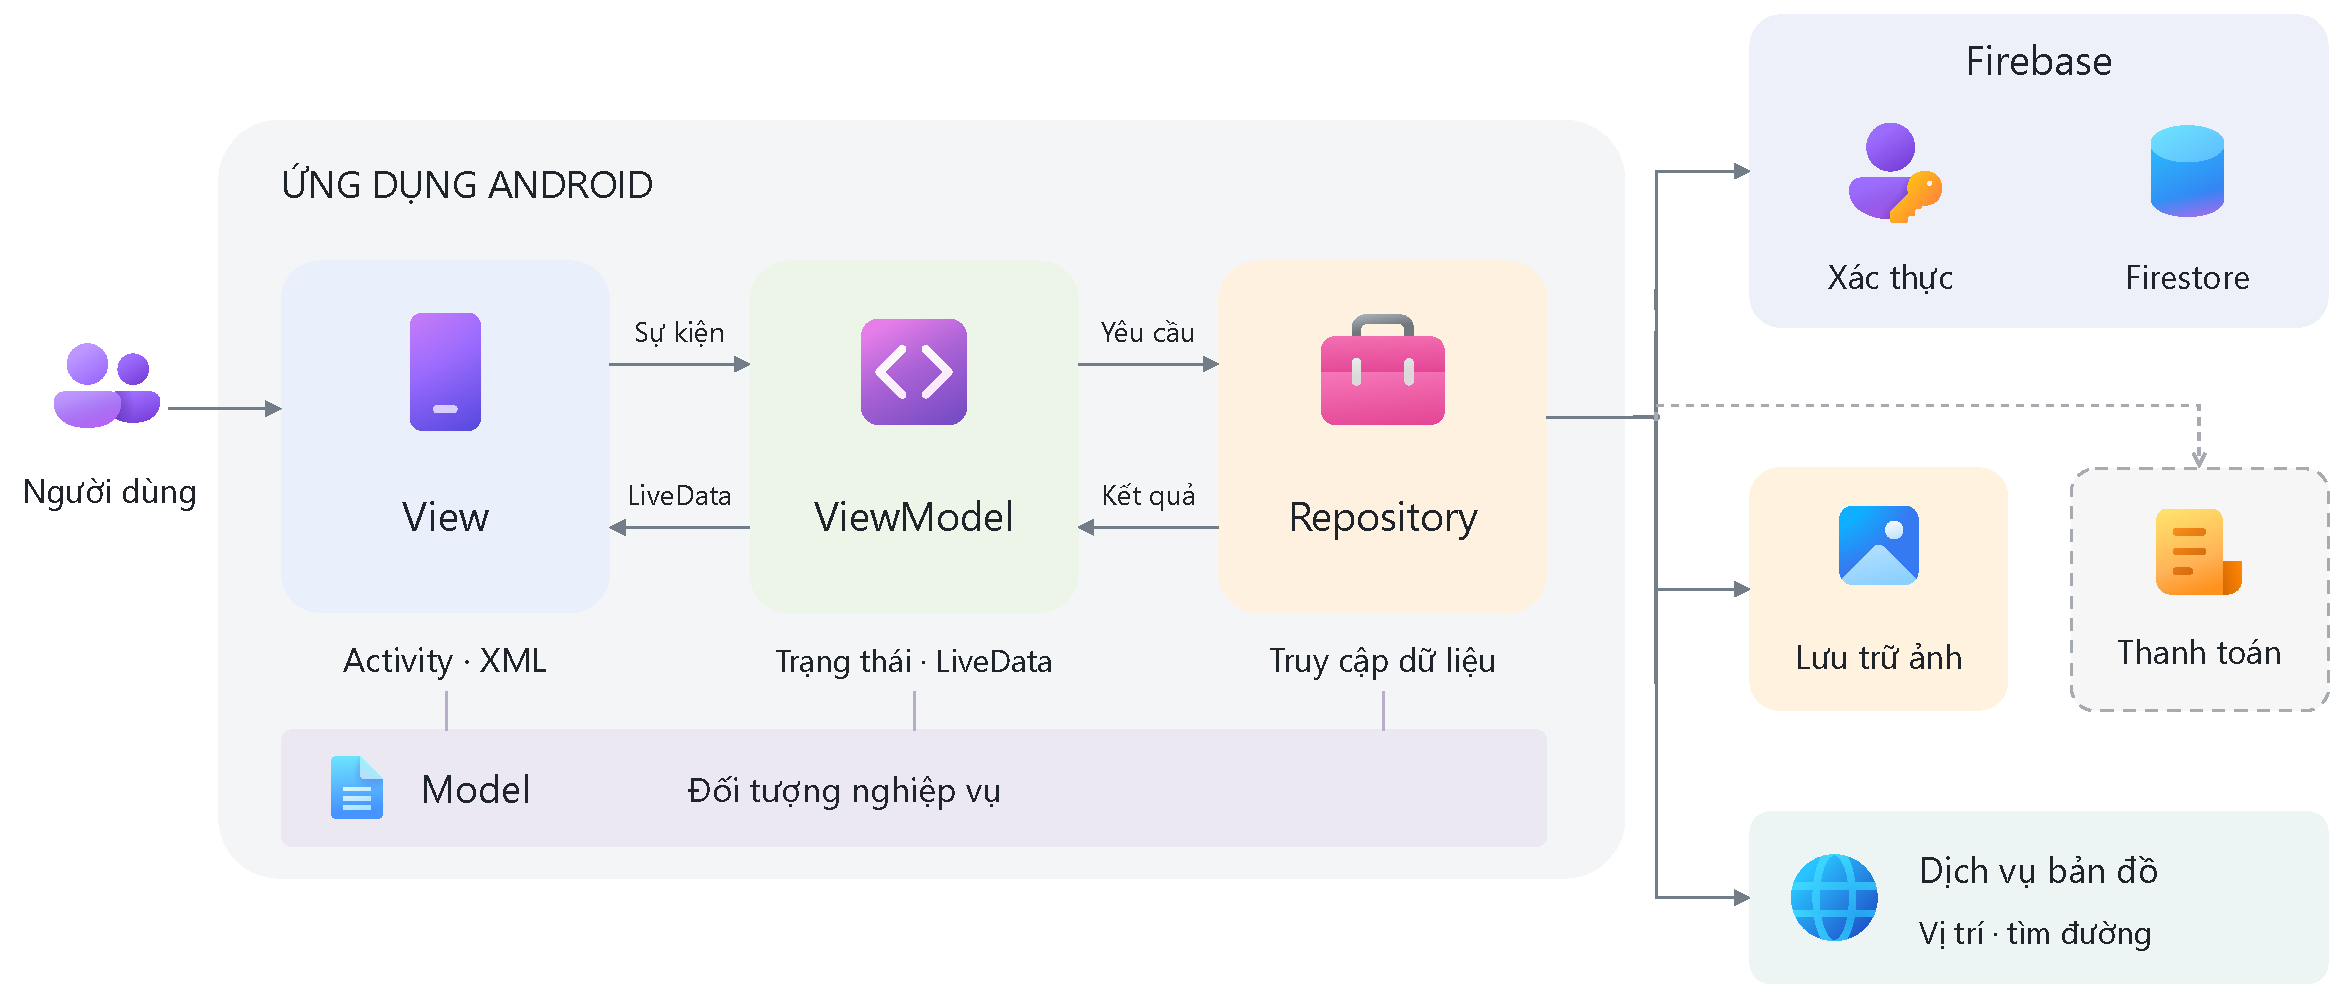
\includegraphics[width=\linewidth]{chapter5/application-architecture.pdf}
\caption{Kiến trúc tổng quan của ứng dụng BroomSharing}
\label{fig:mvvm}
\end{figure}

\subsubsection{Luồng xử lý giữa giao diện và các nguồn dữ liệu}
Activity gửi thao tác tới ViewModel; ViewModel gọi Repository rồi phát trạng thái tải, dữ liệu hoặc lỗi qua LiveData. Chẳng hạn, khi Admin chọn hàng đợi, Repository đọc nhóm hồ sơ tương ứng; khi xét duyệt, dữ liệu được kiểm tra lại trước khi ghi và giao diện chặn gửi lặp trong lúc chờ kết quả.

Với booking, transaction cập nhật đồng thời lượt thuê, lịch và dữ liệu kiểm soát liên quan \parencite{firebase_transaction}. Trạng thái tiền do backend đối soát rồi chuyển tới giao diện qua listener; mở QR hoặc quay về ứng dụng không được xem là đã thanh toán.
